 

\documentclass{article}
%%%%%%%%%%%%%%%%%%%%%%%%%%%%%%%%%%%%%%%%%%%%%%%%%%%%%%%%%%%%%%%%%%%%%%%%%%%%%%%%%%%%%%%%%%%%%%%%%%%%%%%%%%%%%%%%%%%%%%%%%%%%



\usepackage{epigraph}
\usepackage[toc,page]{appendix}

\usepackage{graphicx}
\usepackage{subfig}


\usepackage{multirow}

\newcommand{\ns}{\noindent }

\newcommand{\sh}[1]{\indent\indent\texttt{\footnotesize\$ #1}}
\newcommand{\shni}[1]{\texttt{\footnotesize\$ #1}}


 \textwidth = 400pt
 \textheight = 570pt
 \oddsidemargin =0 pt

\usepackage[colorlinks=true]{hyperref}



\begin{document}

    {\bfseries\Large
        Puebla vs Global temperature trends\\
        \vskip1cm
        R. Angeles\\
    }    




\section{SQL Data extraction}

Check the nearest town using

\sh{SELECT city FROM city-list WHERE country = 'Mexico'}

It is Puebla city. Then the local avg temp timeline can be downloaded from

\sh{SELECT year, avg-temp FROM city-data WHERE city = 'Puebla' }

Finally extract global data 

\sh{SELECT * FROM global-data }

\section{Pandas code}

\begin{figure}[!h]
\centering
  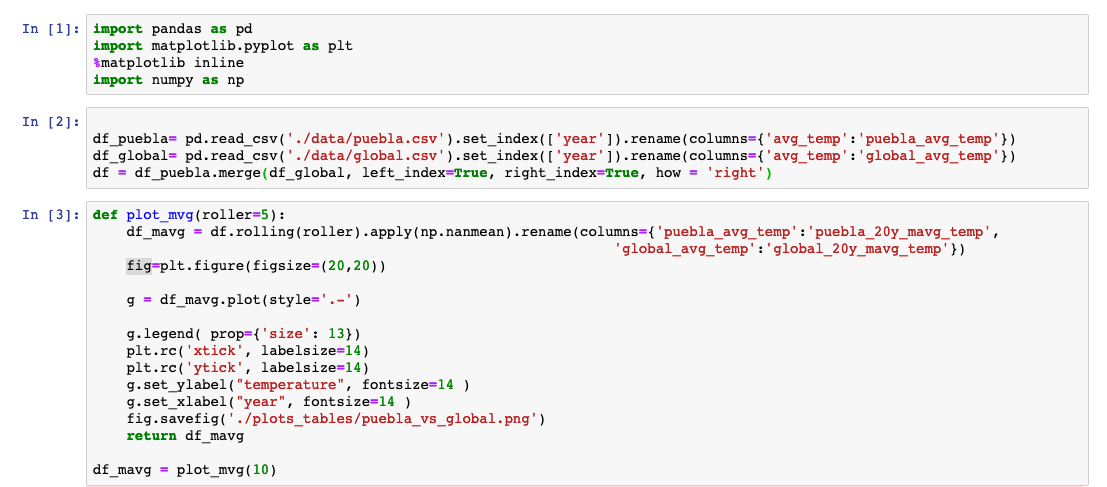
\includegraphics[width=120mm]{../plots_tables/jupyter.png}
%  \caption{Training dataset}
% \label{fig:train_head}
\end{figure}

\section{Running avg temperature}
\begin{figure}[!h]
\centering
  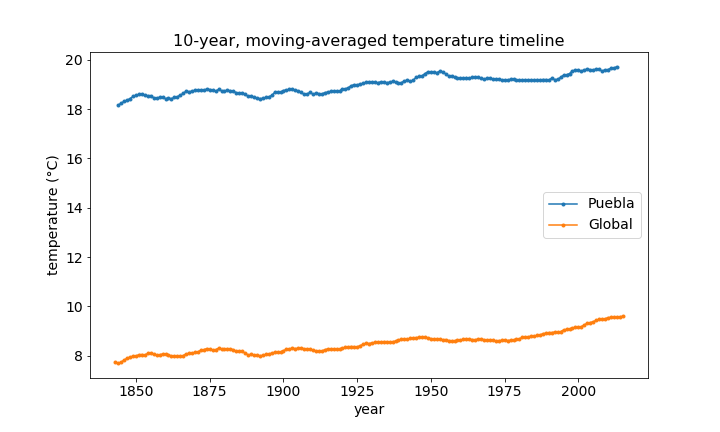
\includegraphics[width=100mm]{../plots_tables/puebla_vs_global.png}
  \caption{10 years running average temperature, time series }\label{fig:vs}
\end{figure}


Observations on  Fig.~\ref{fig:vs}:
\begin{itemize}
\item The year temperature has fluctuations which were tamed by applying 
10 running average but even over 10 years there seems there are fluctuations 
for the global and local case. 
\item Before around 1850 the global temperature fluctuations were larger. 
\item From around 1850  until now the running average seems to be increasing both 
locally and globally. 
\item The largest temperature fluctuations occur globally and before mid 19 century. 
\end{itemize}

\bibliographystyle{unsrt}
\bibliography{qcd22}

\end{document}
